% \begin{frame}{Comparison with \cite{Li26}}
%     \begin{block}{Measured dimensions of alcove}
%     \begin{itemize}
%         \item Length, L
%         \item Width, W
%         \item Vertical thickness, H
%     \end{itemize} 
%     \end{block}

%     \begin{table}
%     \centering
%     \begin{tabular}{lcc}
%     \toprule
%     Metric & This Study & \cite{Li26} \\
%     \midrule
%     $\sqrt[3]{LWH}$ & 1.46 & 1.95 km \\
%     $L/W$       & 3.67 & 0.5--4.25 \\
%     $L/H$       & \alert{4.31} & 1.5--4.0 \\
%     $W/H$       & \alert{1.17} & 1.5--4.0 \\
%     \bottomrule
%     \end{tabular}
%     \caption{Comparison of alcove geometric ratios with averages reported by \cite{Li26}.}
%     \end{table}
% \end{frame}

\begin{frame}{Comparison with \cite{Li26}}

    \begin{columns}[T]
    \begin{column}{0.55\textwidth}

    \begin{block}{Measured dimensions of alcove}
    \begin{itemize}
        \item Length, $L$
        \item Width, $W$
        \item Vertical thickness, $H$
    \end{itemize}
    \end{block}

    \begin{table}
    \centering
    \small
    \begin{tabular}{lcc}
    \toprule
    Metric & This Study & Reference \\
    \midrule
    $\sqrt[3]{LWH}\ (\mathrm{km})$ & 1.46 & 1.95 \\
    $L/W$ & 3.67 & 0.5--4.25 \\
    $L/H$ & 4.31 & 1.5--4.0 \\
    $W/H$ & 1.17 & 1.5--4.0 \\
    Heading & E & S--SE \\
    \bottomrule
    \end{tabular}
    \caption{Comparison of alcove geometric ratios with averages reported by \cite{Li26}.}
    \end{table}

    \end{column}

    \begin{column}{0.45\textwidth}
        \begin{figure}
        \centering
        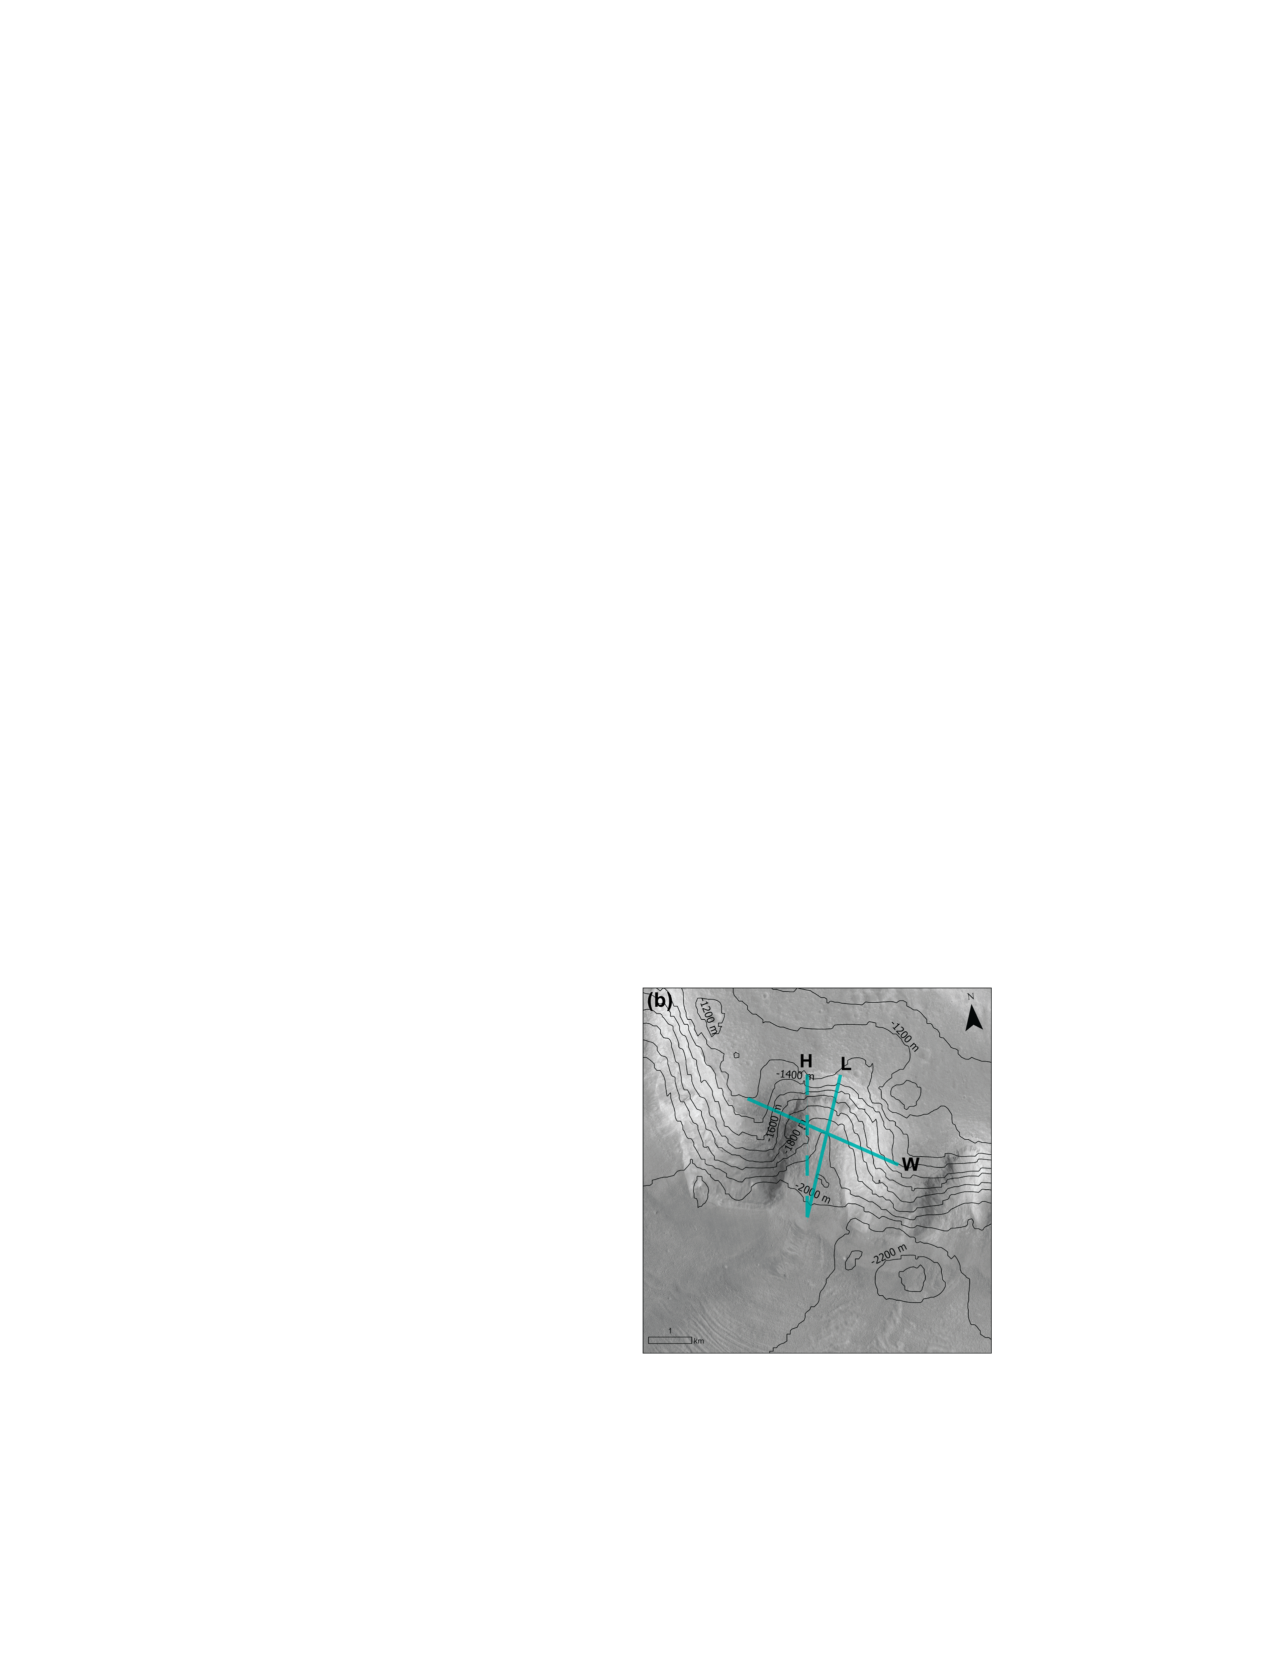
\includegraphics[
            width=\linewidth,
            height=0.6\textheight,
            keepaspectratio
        ]{Figures/Diagrams/Li26_Fig4b.pdf}
        \caption{Definitions of alcove dimensions (Figure from \cite{Li26}).}
        \end{figure}

    % \vspace{0.5em}

    % \scriptsize Alcove dimensions used by \cite{Li26}.
    \end{column}

    \end{columns}

\end{frame}

\section{Conclusions}

\begin{frame}{Main Findings}
    \begin{block}<+->{Evidence that...}
        \begin{itemize}
            \item<+-> Wet-based glaciation was active in Ismenius Cavus.
            \item<+-> Alcove glaciation occurred post-LVF/LDA.
            \item<+-> Sublimation-related features are young.
            \begin{itemize}
                \item Smooth
                \item Few craters
                \item Rubble
            \end{itemize}
        \end{itemize}
    \end{block}
\end{frame}
\begin{frame}{Implications}
    \begin{block}<+->{Geology}
        Wet-based glaciation
        \begin{itemize}
            \item Variable ice content of glacier with depth?
            \item Past geothermal activity?
        \end{itemize}
    \end{block}
    \begin{block}<+->{Climate}
        \begin{itemize}
            \item Alcove creates cooler conditions for stable ice?
            \item Past cooler climate (via $>30^{\circ}$ obliquity)?
        \end{itemize}
    \end{block}
\end{frame}

\begin{frame}{Future Work}
    \begin{block}<+->{Further data needed}
        \begin{itemize}
            \item<+-> Overlapping images $\rightarrow$ DEM analysis.
            \item<+-> Surface investigations to
            \begin{itemize}
                \item Confirm unit relationships.
                \item Confirm activity (or lack thereof).
            \end{itemize}
        \end{itemize}
    \end{block}
\end{frame}